\documentclass[ngerman,pdftex,a4paper,DIV13,12pt,titlepage,fleqn,halfparskip]{scrartcl}


\author{Marc Gebhardt}

\usepackage[utf8]{inputenc}
\usepackage[T1]{fontenc}
\usepackage[ngerman]{babel}
\usepackage{textcomp}\usepackage{lmodern}
%\usepackage{float}
%\restylefloat{table}\restylefloat{figure}
\usepackage{subfigure}
\usepackage{wrapfig}
\usepackage{tabularx}
\newcommand{\changefont}[3]{
\fontfamily{#1} \fontseries{#2} \fontshape{#3} \selectfont}
\usepackage{slashbox}
\usepackage{booktabs}
\usepackage{array}
\usepackage[usenames]{color}
\usepackage{multirow}
\usepackage{paralist}
\usepackage{pict2e}
\usepackage{amsmath}
\usepackage{amssymb}
\usepackage{fancyhdr,graphicx,microtype,ellipsis}
\usepackage[pdfpagemode=UseOutlines,pdftex=true,
	plainpages=false,
	hypertexnames=false,
	pdfpagelabels=true,
	hyperindex=true
	]{hyperref}
	
\pagestyle{fancy}
\lhead{Marc Gebhardt,Albert Möller, Sinja Lagotzki, Sebastian Benecke, Mike Hoffmann}
\chead{}
\rhead{IT2}
\lfoot{27. November 2012}
\cfoot{\thepage}
\rfoot{}
\renewcommand{\headrulewidth}{0.2pt}
\usepackage{pdfpages}
\usepackage[european]{circuitikz}
\usepackage{cite}
\usepackage{paralist} % ist ein erweiterndes Packet für Listen
\usepackage{circuitikz} %für schaltplan!
\usepackage{picins}
\usepackage{wasysym}
\usepackage{pict2e}
\usepackage{lscape}
\usepackage{soul}
\usepackage[right]{eurosym}
\usepackage{array}
\usepackage{multirow}
\usepackage{tikz}
\usetikzlibrary{shapes,arrows}
\title{IT2- Microcontroller Z8}
\subtitle{Praktikum Grundlagen der Informationstechnik}
\author{M. Gebhardt, A. Möller, S. Lagotzki,\\S. Benecke, M. Hoffmann}
\date{27.11.2012}
\publishers{Marc.Gebhardt@st.ovgu.de}
\begin{document}
\maketitle
\changefont{cmss}{m}{n}
\begingroup
%  \renewcommand*{\chapterpagestyle}{empty}
  \pagestyle{empty}
  \tableofcontents
  \newpage
\endgroup  
\setcounter{page}{1}


\section{Einleitung deiner Mutters}
Bei dem Versuch "'Mikrocontroller Z8"' geht es um die hardwarenahe Bedienung und Programmierung des 8-Bit-Microcontrollers Z8 der Firma Zilog. Dazu gehört das Kennenlernen der Hardwarestruktur und des Befehlssatzes des Mikrocontrollers, sowie Aneignung von Grundlagen der Assembler-Programmierung und das Ausführen der geschriebenen Programme. 

\section{Versuchsaufbauhauhauhau}
hahahahahahuhuhu
An den Arbeitsplätzen waren PCs mit der Software für die Programmierung des Assemblercodes vorhanden. Es wurde das Zilog Developer Studio I (ZDS 3.68) verwendet, das den Zilog Macro Cross Assembler (ZMASM) sowie ein Debug-Interface zur Verfügung stellt, was zusammen mit dem Emulator "'Z86CCP00ZEM"' die Möglichkeit der interaktiven Entwicklung von Applikations-Software darstellt. Der Emulator ist an den PC angeschlossenen und über ein Adapterkabel mit der User-Platine verbunden. Dort ersetzt er den tatsächlichen Mikrocontroller, bringt aber die selben Eigenschaften mit. Bei dem Z86CCP00ZEM sind das:
\begin{compactitem} 
\item 20 MHz, Z86C50-20FSE Emulations-Controller
\item 8kByte Emulationsspeicher
\item 256 8-Bit-Register
\item 4 8-Bit Ports
\item 2 Programmierbare 8-bit Counter/Timer mit Vorteiler 
\item 6Vektorisierte priorisierbare Interrupts
\item 8 MHz Emulation-Speed
\item 2 programmierbare Analogeingänge
\item 256 Setzbare Breakpoints
\item Target-Sockets: 18-Pin, 28-Pin, 40-Pin
\end{compactitem}
Auf der User-Platine konnten die Ergebnisse der programmierten Aufgaben verfolgt werden. Die 4 Ports des Emulators waren mit LEDs, bzw Schaltern verbunden, um die Ein- und Ausgabe umzusetzten und zu beobachten, außerdem konnte der Verlauf von Signalen mit Hilfe eines Oszilloskops aufgezeichnet werden. 

\section{Versuchsdurchführung, Beobachtung und Auswertung}
\subsection{Port 1-Komplex}
\subsubsection{Speichererweiterung}

Es gibt einen externen und einen internen RAM, sowie einen externen und einen internen ROM.
RAM bedeutet Random Access Memory. Auf diesen Speicher kann direkt zugegriffen werden.
ROM steht für read-only Memory, was bedeutet, dass dieser Speicher nur lesbar ist und nicht beschrieben werden kann. Es handelt sich somit um einen nicht flüchtigen Speicher.
Der Interne RAM ist $2^8=256$ Byte groß. Die Register 0-3 sind für die Ports vorgesehen, diese Register können also nicht verwendet werden, um Adressen oder Werte zu speichern.
Im Z8 nimmt der interne ROM $2^{12}=4096$Byte (FFF) ein und der externe ROM reicht von dort bis zur $2^16=65535$Byte-Marke (FFFF). Der externe RAM ist ähnlich aufgebaut. Es gibt wieder einen Bereich von $0$ bis $2^{12}$, der hier allerdings auf „not avaiable“ gesetzt ist. Dieser Bereich überlagert sich mit dem internen ROM. Der restliche Speicherplatz aus dem externen RAM besteht zunächst aus nicht benutzbaren Teilen A8-A12. Es bleiben letztlich $2^8$ Byte übrig, in dem die Werte abgespeichert werden können. Es stellt sich nun die Frage, wo findet sich dieser Speicher in den 60kB wieder? 28Enspricht etwa $\frac{1}{4}$ kB, somit passt dies in die 60kB genau 240 Mal. Der RAM wird also immer wieder gespiegelt. Dies geschieht von den Adressen 1000 – FFFF, denn die beiden  ersten Stellen werden vom  Speicher nicht mehr gesehen und alles wird gespiegelt.
Der RAM war nun zu testen, dazu wurde einmal die Spiegelung getestet und zusätzlich geschaut, ob die Werte richtig geschrieben und gelesen werden, indem man während der Laufzeit die Änderungen der Register beobachtet.

Das Programm sieht folgendermaßen aus:
\begin{verbatim}
org %0C					        Die Anfangsadresse wird definiert
ld P01M, #%10			  Die Ports werden initialisiert.

ld R4, #%AB				    Das Bitmuster wird festgelegt und in ein Register geladen.

ld R6, #%12				    Der High-Teil wird nun in ein gerade Register geladen,
ld R7, #%34				    während der Low-Teil ins ungerade Register geladen wird.

lde @RR6, R4			   Es wird nun das Bitmuster in den externen RAM geschrieben. 
									                Dies macht man, indem man Doppelregister verwendet. @RR6 
					                steht für das Register 6 und das nachfolgende, 
					                also Register 7. 							
					                Das Bitmuster wird also nun auf die in R6 und R7 gespeicherte 		
						                Adresse geschrieben.

ld R6, #%23				    Nun wird der High-Teil geändert, denn daran ist zu erkennen, 
                ob die Spiegelung erfolgt.
lde R5, @RR6			   Als nächstes wird vom externen RAM gelesen.

ld R8, #%CD				    Der gleiche Ablauf wird nun noch einmal mit einem zweiten
 	              Bitmuster durchgeführt.
ld R6, #%45				    Es wird wieder der High-Teil geändert.
lde @RR6, R8			   Der nächste Schritt ist das Schreiben in den externen RAM
ld R6, #%67				    und das erneute ändern des High-Teils.
lde R9, @RR6			   Nun wird der RAM erneut ausgelesen.
\end{verbatim}

\subsubsection{Programmierung eines externen Stacks}

Es muss zunächst das richtige Steuerwort für Port 1 errechnet werden. Dies ist das selbe wie in 3.1.1, nämlich 10h.

\begin{verbatim}
org %0C                   Starten des Hauptprogramms an Adresse 0C
ld P01M,#%10              Konfigurieren von Port 1
ld sph,#%10               Oberer Addressteil des Stackpointers
ld spl,#%80               Oberer Addressteil des Stackpointers
call %500                 Aufruf der Adresse 500h
LOOP: jp LOOP             Endlosschleife am Programmende

org %500                  Start des Unterprogrammes an Stelle 500h
call %600                 Aufruf der Adresse 500h
ret                       Rückkehr zum Hauptprogramm

org %600                  Start des Unterprogrammes an Stelle 600h
ret                       Rückkehr zum ersten Unterprogramm
\end{verbatim}

Der Port 1 wird also als externer Speicher konfiguriert und der Stackpointer an dessen Position 1080h gesetzt. Dann wird auf das Unterprogramm an der Stelle 500h gesprungen, dabei wird die Addresse von der gesprungen wurde (0018h) auf den Stack geschoben und taucht  auf Stackadresse 1080h auf. Dann wird Adresse 600h aufgerufen und die Adresse von der gesprungen wurde wieder auf den Stack gerettet. Diesmal auf die Stackadresse 1079h. Demnach ist der Stack ein Tiefstapler da neue Stackeinträge eine niedrigere Stackadresse haben.

Durch die Return-Befehle wird immer wieder auf die vorhergehenden Programme zurückgesprungen. Dabei wird erst die Adresse 0503h von der Stackadresse 1079h geladen und dann die Adresse wo im Hauptprogramm unterbrochen wurde (0018h) aus dem Beginn des Stacks bei 1080h.

\newpage


\subsection{Port0-/Port2-Komplex}

\textbf{Teil a}

Zu entwickeln war ein Programm, welches zyklisch die an Port 2 angeschlossenen Schalter abfragt und die Schaltzustände an Port 0 ausgibt.
Zunächst geben wir die Startadresse des Programms an. Hier 0Chex (12dez). Danach müssen die Ports mit den entsprechenden Steuerwörtern initialisiert werden.
Steuerwörter der Ports:
Für Port 0 (Ausgabe) müssen die Bits D7, D6, D1 und D0 auf 0 gesetzt sein. Die anderen Bits sind hier nicht relevant und werden auf 0 gesetzt. Es ergibt sich ein hexadezimales Steuerwort für P0 von 00. Bei Port 2 geben alle Bits die Funktionsweise an. Wenn diese auf nur 1 gesetzt sind, arbeitet der Port als Eingabe. Somit ergibt sich das Steuerwort für Port 2 FF.

Nun folgt die Schleife mit dem einlesen von Port 2 und ausgeben an Port 0. Dafür wird der Wert an Port 2 in R4 gespeichert  und anschließend R4 in Port 0 ausgegeben. Als Letztes kommt der Sprung zurück zum Punkt M, welcher direkt vor dem einlesen von Port 2 liegt.

\begin{verbatim}
org %0C
ld  P01M, #%00
	ld P2M, #%FF
M:	ld R4, P2
	ld P0, R4
	jp M
\end{verbatim}

\textbf{Teil a-Zusatz}

Es sollte eine Schaltkombination an Port 2 eingelesen und an P0 ausgegeben werden.
Als Zusatz zur Aufgabe sollte die Reihenfolge der angehenden Leuchten geändert werden, sodass, bitweise betrachtet, das Bit D7 zu D0 wird, D6 zu D1 und analog für die anderen Stellen weiter damit die richtige Reihenfolge gewährleistet wird.
Es wurde die Methode des Testens auf Maske gewählt. So kann bitweise das eingelesene Register vertauscht werden. Es wird der Reihe nach jede Stelle auf 80(\textbf{1}000000), 40, 20, 10, 08, 04, 02, 01 geprüft. Wenn nun das erste Bit (D7) eine 1 trägt, so wird im neuen Ausgaberegister eine 1 an die letzte Stelle (D0) gesetzt. So geht man alle acht Stellen durch und erhält im neuen Register dann die neue Dualzahl, in der nun die Einsen und Nullen gegen Nullen und Einsen getauscht wurden.

\textbf{Steuerwörter der Ports}
Für Port 0 (Ausgabe) müssen die Bits D7,D6,D1 und D0 auf 0 gesetzt sein. Die anderen Bits sind hier nicht relevant und werden auf 0 gesetzt. Es ergibt sich ein hexadezimales Steuerwort für P0 von 00.
Bei Port 2 geben alle Bits die Funktionsweise an. Wenn nur 1 gesetzt sind, arbeitet der Port als Eingabe.
\begin{verbatim}
	org %OC
	ld P01M,#%00
	ld P2M, #%FF
S:  ld R4, P2

	ld R5,#%00
	TM R4,#%01
	jp z,M
	OR R5,#%80
M:  TM R4,#%02
	jp z,M1
	OR R5,#%40
M1: TM R4,#%04
	jp z,M2
	OR R5,#%20
M2: TM R4,#%08
	jp z,M3
	OR R5,#%10
M3: TM R4,#%10
	jp z,M4
	OR R5,#%08
M4: TM R4,#%20
	jp z,M5
	OR R5,#%04
M5: TM R4,#%40
	jp z,M6
	OR R5,#%02
M6: TM R4,#%80
	jp z,M1
	OR R5,#%01
	
M7: nop				
	ld P0,R5
	jp S	
\end{verbatim}
Es kann erst ab Speicheradresse 12 geschrieben werden, da die Adressen 0-11 anderweitig (Interrupt) genutzt werden. Nun werden die Ports mit den vorher ermittelten Steuerwörtern definiert und der Eintrag von Port2 auf das Register R4 kopiert.
Nun startet das Umkehren des Registers, indem wir ein neues Register (R5) hinzunehmen und dieses auf 00 setzen. Um den Vergleich am ersten Schritt zu erklären denken wir uns im ersten Fall im 0. Bit eine 1. Dann wird mit 00000001 getestet und erkannt, dass die Zahlen gleich sind. So meldet der Maskentest eine 1. Da es keine Null ist, ist der Jump-Befehl ergebnislos. Es wird nun durch den OR-Befehl in das Register 5 eine 1 an erste Stelle, also ins 7. Bit geschrieben. Wäre im zu testenden Register R4 eine Null an letzter Stelle eine Null, so hätte der Maskentest eine Null geliefert und das Programm hätte via Jump die Erstellung der 1 an 1. Stelle im neuen Register übersprungen.
Analog zu dieser Syntax läuft das Programm alle Stellen ab.
Man könnte das Programm auch mit Schleifen und/oder Tabellen betreiben, wobei die Effizienz der Arbeitsschritte in diesem Falle im Hintergrund stehen sollte. Zum Schluss wird das neu befüllte Register 5 an Port 0 ausgegeben.
$\rightarrow$ Nach Durchführung des Programms am PC mit kalibriertem Microcontroller ließen sich nun die Leuchten in richtiger Reihenfolge schalten.

\newpage
\textbf{Teil b - Lauflicht}

Wie bereits in der vorigen Aufgabe wird wieder mit den Ein- Ausgabeports 0 und 2 gearbeitet. Hierbei sollten beide Ports der Ausgabe dienen und mittels der LEDs, die an den Pins der Ports angeschlossen sind, ein Lauflicht betrieben werden. Damit ein Lauflicht zu beobachten ist, muss jedes Licht eine bestimmte Zeit leuchten. Da der Emulationscontroller mit einem Takt von 20 MHz läuft, sollte jeder Pin für etwa 120000 Operationen angesteuert sein, um eine Leuchtzeit von etwa einer halben Sekunde zu erreichen.\\


\tikzstyle{decision} = [diamond, draw, fill=blue!20, 
    text width=4.5em, text badly centered, node distance=3cm, inner sep=0pt]
\tikzstyle{block} = [rectangle, draw, fill=blue!20, 
    text width=6em, text centered, rounded corners, minimum height=4em]
\tikzstyle{line} = [draw, -latex']
\tikzstyle{cloud} = [draw, ellipse,fill=red!20, node distance=3cm,
    minimum height=2em]
    
\begin{figure}[h!]
\begin{tikzpicture}[node distance = 2cm, auto]
	% Place nodes
	\node [block] (init) {Ports initialisieren};
	\node [block, below of=init] (licht1) {erste LED einschalten};
	\node [block, below of=licht1] (warten1) {Warteschleife};
	\node [block, below of=warten1] (licht2) {nächste LED einschalten};
	\node [block, left of=licht2, node distance=3cm] (warten2) {Warteschleife};
	\node [decision, below of=licht2] (entsch1) {letzter Ausgang des Ports?};
	\node [block, right of=licht1, node distance=3cm] (nächster) {anderen Port ansteuern};
   	 % Draw edges
	\path [line] (init) -- (licht1);
	\path [line] (licht1) -- (warten1);
	\path [line] (warten1) -- (licht2);
	\path [line] (licht2) -- (entsch1);
	\path [line] (entsch1) -| node [near start]{ja} (nächster);
	\path [line] (entsch1) -| node [near start]{nein} (warten2);
	\path [line] (warten2) -- (licht2);
	\path [line] (nächster) -- (licht1);
\end{tikzpicture}
\caption{Programmablaufplan: Lauflicht}\label{pap32}
\end{figure}

Der Programmablaufplan (Abbildung \ref{pap32}) verdeutlicht das grundlegende Konzept für das Lauflicht. Es wird nacheinander jedes Bit der Ports aktiviert und gleichzeitig muss das gerade aktivierte Bit ausgeschaltet werden. \\\\
Die erste Zeile des Assamblercodes legt wie üblich die Startadresse, wo der erzeugte Maschinencode in den Emulator-RAM geladen wird, fest. Danach werden die Ports entsprechend ihrer Aufgabe konfiguriert. Da hier Port 0 und Port 2 als Ausgabe dienen, müssen sie beide mit dem Steuerwort 00h initialisiert werden. Dazu wird ebenfalls der Port 3 mit 01h initialisiert. Dies ist notwendig, da an dem Ausgang von Port 2 keine aktiven Geräte angeschlossen sind. Wenn das erste Bit in dem Steuerwort für Port 3 eins gesetzt ist, sind Pull-ups für den zweiten Port aktiviert, die dafür sorgen, dass die Information für ein high auf den Bits nicht verloren geht, selbst wenn für die Ausgabe kein aktives Gerät vorhanden ist, also ein hochohmiger Zustand vorliegt.\\
Die Steuerwörter werden dann mit dem Befehl "'ld"' in das Steuerregister des jeweiligen Ports geschrieben (P01M für Port0, P2M für Port2 und P3M für Port 3). Damit kann man dann über Port und und Port 2 Signale ausgeben, indem man Daten in Register R0 und R2 läd ("'ld R0,--"' ;"'ld R2,--"'). Da das Lauflicht nicht nach einem Durchlauf aufhören sollte, sondern immer wieder von vorn anfangen, kommt nach der Initialisierung der Ports die Sprungmarke "'S3:"'. Darauf folgt das Ausschalten aller LEDs auf Port 1 und das Setzen eines Sprungzählers in R4 auf acht. In den acht Sprüngen wird jeweils das aktive Bit des Registers um eine Stelle nach rechts geschoben ("'rr R0"'). Vor der Sprungmarke "'S1:"' für die Schleife, muss jedoch noch mit dem Befehl "'ld R0,$\#\%80$"'  das achte Bit von Port 00 auf 1 gesetzt werden.\\\\

Innerhalb jedes Durchlaufs der Schleife S1 wird die Warteschleife W1 abgearbeitet. Das Prinzip der Schleife verdeutlicht Abbildung \ref{Zählschleife}. Beim Beginn von S2 wird die Zahl 255 in R6 und R8 geladen, und dann bis null runtergezählt. Umgesetzte ist dies mit dem Befehl "'djnz R6,W1"' für beide Register und einem "'nop"' am Anfang der Schleife W1. Damit werden zwar lediglich zwei mal 510, also 1020 Zeillen Code in der Warteschleife abgearbeitet, aber die Leuchtzeit war ausreichend lang, was darauf schließen lässt, dass der Prozessor weitaus mehr Operationen zum Ausführen des Codes benötigt. Wenn die Warteschleife(siehe Abbildung \ref{Zählschleife} auf Seite \pageref{Zählschleife}) noch nicht ausreichend gewesen wäre, ist es noch möglich bei dem Runterzählen von R8, R6 jedes mal wieder auf 255 zu stellen, damit es für jeden Wert von R8 noch einmal von 255 bis null dekrementiert wird. Damit wären dann 255 mal 510, also 130050 Codezeilen abgearbeitet worden.\\

 \begin{figure}[!ht]
\centering % centering figure
\scalebox{0.5} % rescale the figure by a factor of 0.8
{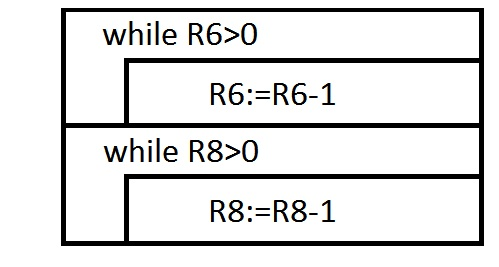
\includegraphics{struk32.jpg}} % importing figure
\caption{Ablauf der Warteschleife} \label{Zählschleife}
\end{figure}

Wenn dann zum achten mal der Sprung auf S2 erfolgt ist, geht der Prozessor aus dieser Schleife raus und es werden alle Lichter an Port 0 ausgeschaltet sowie das erste Bit an Port 2 auf 1 gesetzt ("'ld R2,$\#\%01$). Daraufhin folgt der selbe Ablauf wie von Port 1 mit einem kleinen Unterschied. Da die Lichter an Port 2 in umgekehrter Reihenfolge angeschlossen sind wie an Port 0, muss für ein Lauflicht in die gleiche Richtung das aktivierte Bit nach links anstatt rechts verschoben werden. Es wird somit der Befehl "'rl R2"' verwendet. Außerdem wird der Schleifenzähler für S2 nur auf 7 anstatt auf 8 gesetzt, da nach dem letzten Durchlauf noch einmal das Bit um eins nach links verschoben wird, gefolgt von einer Warteschleife. Dieser Zeilen hätten allerdings mit einem weiteren Sprung auf S2 eingespart werden können. Dann werden wiederum alle Bits von Port 2 auf null gesetzt. Beendet wird der Assemblercode mit einem unkonditionierten Rücksprung auf S3 ("'jp S3"'), was eine Endlosschleife zur Folge hat, und abschließend wird ein nop gesetzt, was lediglich einen notwendigen Befehl für den Assembler darstellt.\\
Der komplette Code für das Programm sieht dann wie folgt aus:

\begin{verbatim}
   org 0ch
   ld P01M,#%00
   ld P2M,#%00
   ld P3M,#%01
S3:ld R0,#%00
   ld R4,#%8
   ld R0,#%80
S1:ld R6,#255
   ld R8,#255
W1:nop
   djnz R6,W1
W2:djnz R8,W1
   rr R0
   djnz R4,S1
   ld R0,#%00
   ld R2,#%01
   ld R4,#7
S2:ld R6,#255
   ld R8,#255
W3:nop
   djnz R6,W3
W4:djnz R6,W3
   rl R2
   djnz R4,S2
   ld R6,#255
   ld R8,#255
W5:nop 
   djnz R6,W5
W6:djnz R8,W5
   rlc R2
   ld R2,#%00
   jp S3
   nop
\end{verbatim}

\textbf{Teil c: Zählung der Schaltvorgänge an Port 2}

Bei dieser zusätzlichen Aufgabe sollte an Port 0 binär die Anzahl der Schaltvorgänge an Port 2 ausgegeben werden. Dabei trat das Problem auf, dass bei manchen Schaltvorgängen diese mehrfach gezählt wurden. Dies trat auf, da die Schalter nicht entprellt waren und so im Bruchteil einer Sekunde zwischen zwei Zuständen hin und her sprangen. Daher wurde nachträglich ein Zählschleife eingeführt, welche bewirkt das zwischen zwei Messungen mehr Zeit liegt und die Schalter auf ihrer schlussendlichen Position angekommen sind. Allerdings kann es dadurch vorkommen, dass wenn sehr schnelle hin und her Schaltvorgänge während der Zählschleife auftreten, diese nicht gezählt werden. 

Unser Quellcode:

\begin{verbatim}
org 0Ch               Beginn der Hauptprogramms                
ld P01M,#%00          Konfigurierung von Port 0
ld P2M,#%FF           Konfigurierung von Port 2
ld P0,#0              Löschen aller Lichter an Port 0 
ld R6,P2              Einlesen des Wertes von P2
ld R8,#%0             Register 8 Null setzen

Nachträglich eingefügte Zählschleife
M: ld R7,#%FF         Register 7 auf den Wert FFh setzen
N: djnz R7,N          Register 7 um 1 erniedrigen und wenn es 
                      nicht Null ist zu M springen

ld R4,P2              Einlesen von Port 2 auf Register 4
cp R4,R6              Vergleichen von R4 und R6 
                      Vorheriger Wert zu jetzigem Wert
                      Sind sie gleich wird das Zero-Flag gesetzt
jp Z,M                Bei gesetztem Zero-Flag Sprung zu M
                      D.h. Port 2 wird neu abgefragt und Port 0 bleibt gleich
ld R6,R4              Jetziger Wert wird zu Vorherigem Wert beim nächstem Durchlauf
add R8,#%01           Register 8 wird um 1 erhöht
ld P0,R8              Register R8 wird ausgegeben
jp M                  Sprung zu M es folgt eine neue Abfrage von Port 2
\end{verbatim}

Zu Anfang werden also alle Lichter am Port 0 gelöscht, da es ja noch keine Schaltvorgänge gab. Dann wird einmalig der Wert von P2 auf das Register 6 (Vorheriger Zustand von P2) geladen, damit beim ersten Durchlauf der Auswertschleife kein Schaltvorgang erkannt wird. Das Zählregister R8 wird Null gesetzt. Nach dem Durchlaufen der Verzögerungsschleife wird auf R4 (Jetzt Zustand von P2) der aktuelle Wert von P2 geladen. Vorheriger Zustand und jetziger Zustand werden verglichen um festzustellen ob sie sich geändert haben. Sind sie gleich wird das Zero-Flag gesetzt, sonst gelöscht. Beim darauf folgendem Jump Befehl wird zu M gesprungen, falls das Zero-Flag gesetzt ist. Es ist dann also kein Schaltvorgang aufgetreten da der vorherige und  der jetzige Wert gleich sind. Daher wird P2 wieder neu abgefragt. Ist das Zero-Flag nicht gesetzt, läuft das Programm normal weiter, da es einen Schaltvorgang gegeben hat. Der jetzige Wert R4 wird zum vorherigem Wert R6 für den nächsten Durchlauf. Das Zählregister R8 wird um 1 erhöht und auf Port 0 ausgegeben. Dann wird zurück zu M gesprungen und P2 erneut abgefragt.

\subsection{war nicht zu bearbeiten}


\subsection{Timer 1-Komplex}
\textbf{Teil a}
\begin{figure}[!ht]
\begin{center}
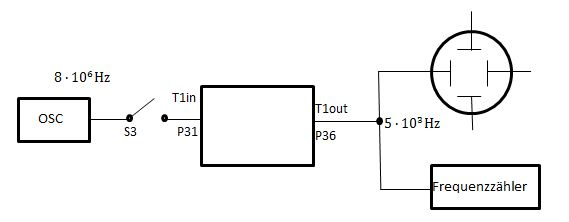
\includegraphics[width=0.75\textwidth]{34a1} 
\caption{Frequenzschema 3.4 a}
\label{341a}
\end{center}
\end{figure}

Mit Anlage 5 kommen wir zu folgender  Vereinfachung zur die Berechnung der Ausgangsfrequenz.


\begin{figure}[!ht]
\begin{center}
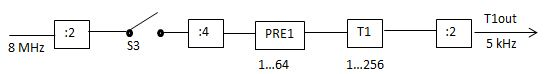
\includegraphics[width=0.75\textwidth]{34a2} 
\caption{Optionen der Einstellung 3.4 a}
\label{34a1}
\end{center}
\end{figure}


Berechnung der nötigen Werte für PRE1 und T1:
\begin{align*}
\frac{8\cdot 10^6}{2\cdot4\cdot2\cdot\text{Pre1}\cdot\text{T1}}&=5\cdot10^{-3}\\
\text{Pre1}\cdot\text{T1}&= \frac{8\cdot10^6}{2\cdot4\cdot2\cdot5\cdot10^3}
\end{align*}
Somit muss das Produkt aus Prescaler und Timer 100 ergeben um die 5 kHz an T1out zu erhalten. Gewählt wurde hier für beide der Wert 10. Daraus ergeben sich die Steuerworte 29hex für den Prescaler(PRE1) und 0Ahex für den Timer(T1). 29hex ergibt sich aus D0=0 für Modulo N, D1=0 für External Timing und D2 bis D7 enthalten den Teilerwert des Prescalers als Binärzahl (hier: 001010bi). 0Ahex ist einfach nur der Teilerwert des Timers als Binomialzahl.
Zuvor werden Port 2 mit dem Steuerwort 00hex (Steuerregister P3M)und  Timer Mode(TMR) mit dem Steuerwort 9Chex initialisiert. Für Port 2 war nur D5 von Belang, da dieses  beim Inhalt  Null P31 als Input(Tin) und  P36 als Output(Tout) initialisiert. Für den Timer Mode ergibt sich das Steuerwort aus D2=1 für Load T1, D3=1 für Enable T1 Count, D4 D5 =01 für P31 als Gate Input und D6 D7=10 für P36 als T1out.D0 und D1 hätte bei dem Wert Eins T0 konfiguriert, welche hie nicht von nötig war, somit wurden diese auf Null gesetzt.
Zum Schluss folgen die Sprungmarke S1 und einem Sprungbefehl zu S1, welche verhindern dass das Programm nicht beendet wird bzw.  andere im Speicher liegende Befehle ausführt.

\begin{verbatim}
org %0C
ld P3M, #%00
ld TMR, #%9C
ld PRE1, #%29
ld T1, #%0A
S1:
	jp S1
\end{verbatim}
Messung mit dem Oszilloskop: $T= 200\mu s $ mit $f=\frac{1}{T}$ ergibt sich die gemessene Frequenz $f=5 kHz$

Messung mit digitalem Frequenzzähler: $f=5,003 Hz$


\begin{figure}[!ht]
\begin{center}
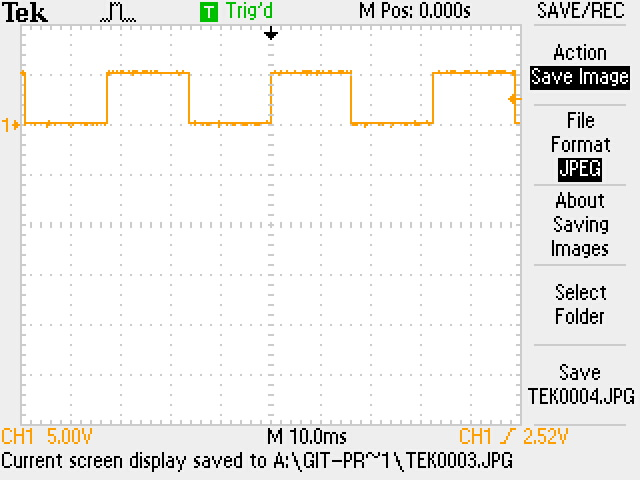
\includegraphics[width=0.75\textwidth]{os1} 
\caption{Oszillogramm mit eingeschaltetem Schalter am Port 2}
\label{os34a1}
\end{center}
\end{figure}


\begin{figure}[!ht]
\begin{center}
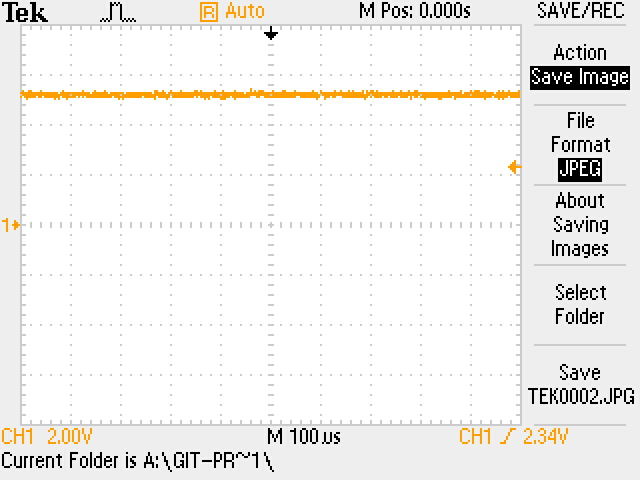
\includegraphics[width=0.75\textwidth]{os2} 
\caption{Oszillogramm mit mit ausgeschaltetem Schalter am Port 2}
\label{os34a2}
\end{center}
\end{figure}


\newpage

\textbf{Teil b:}

Es sollte der Timer 1 als Frequenzteiler(siehe Abbildung \ref{34bv} auf Seite \pageref{34bv}) für eine an P31 ($T1_{IN}$) anliegende Impulsfolge(1 MHz) verwendet werden. Durch Frequenzmessgerät und Oszi sollte der kleinste und größte Teilerfaktor gemessen werden und dann mit dem berechneten Wert verglichen werden.

\begin{figure}[!ht]
\begin{center}
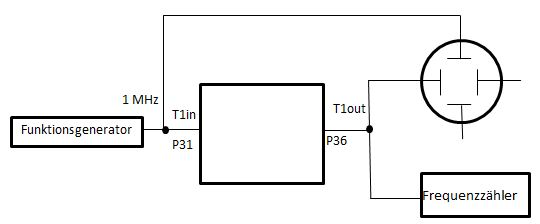
\includegraphics[width=0.75\textwidth]{34bv} 
\caption{schematischer Versuchsaufbau}
\label{34bv}
\end{center}
\end{figure}


\textbf{Port-, Timer- und Prescalerdefinitionen}
Für Port 3 übernehmen wir das Steuerwort aus 3.4 a) als 00hex.

Für das Timermoderegister (R241) ermitteln wir: \textbf{1000 1100}
D7 und D6 sind 10, da T1 als Input genommen wird.
Da der Takt extern vorgegeben wird, werden D5 und D4 null gesetzt.
Mit D3=1 und D2=1 wird T1 als Eingang aktiviert.
D1 und D0 werden, da sie hier nicht genutzt werden auch auf 0 gesetzt.
Es ergibt sich ein Steuerwort 8Chex.

\begin{figure}[!ht]
\begin{center}
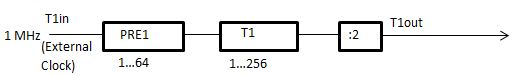
\includegraphics[width=0.75\textwidth]{34bs} 
\caption{Teilererzeugung}
\label{34bs}
\end{center}
\end{figure}


Für den Timer T1 erkennt man ein Teilerspektrum von 1 bis 256, wobei das 00hex(0000000\textbf{0}) den Teiler 256 darstellt und 01hex(0000000\textbf{1}) den Teiler 1.

Für den Prescaler gilt:
Es werden D1 und D0 wie in 3.4a als 01 gesetzt.
Die Bits D7-D2 legen den Teilerfaktor fest, wobei der maximale Faktor mit 01hex (00000\textbf{0}01 realisiert wird und der Minimale mit05hex (00000\textbf{1}01.
(siehe Abbildung \ref{34bs} auf Seite \pageref{34bs})
\begin{verbatim}
org %0C
ld P3M,#%00
ld TMR,#%8C

1. größter Teiler: 
ld PRE,#%01
ld TMR,#%00

2. mittelerer Teiler 1:
ld PRE,#%05
ld TMR,#%00

3. mittelerer Teiler 2: 
ld PRE,#%01
ld TMR,#%01

4. kleinster Teiler: 
ld PRE,#%05
ld TMR,#%01

S1: jp S1
\end{verbatim}
Nach Messung erhalten wir: \newline
$f_1=30,52 Hz$\newline
$f_2=1,95376 kHz$\newline
$f_3=7,81 kHz$\newline
$f_4=500,16 kHz$\newline
Zum Vergleich berechnen wir die Frequenzen mit:
\begin{align}
f&=\frac{1 MHz}{Prescaler\cdot Timer \cdot 2} \\
\mathsf{1.}&\nonumber\\
f&=\frac{1 MHz}{64\cdot 256 \cdot 2}= 30,516 Hz\\
\mathsf{2.}&\nonumber\\
f&=\frac{1 MHz}{1\cdot 256 \cdot 2}= 1,953123 kHz\\
\mathsf{3.}&\nonumber\\
f&=\frac{1 MHz}{64\cdot 1 \cdot 2}= 7,8125 kHz \\
\mathsf{4.}&\nonumber\\
f&=\frac{1 MHz}{64\cdot 256 \cdot 2}= 30,516 500 kHz
\end{align}


\begin{table}[!ht]
\begin{center}
\begin{tabular}{||c|c|c||}
\hline 
\rule[-1ex]{0pt}{2.5ex} Variante & $f_{Mess}$ & $f_{Rechnung}$ \\ 
\hline 
\rule[-1ex]{0pt}{2.5ex} 1& 30,52 kHz & 30,516 Hz \\ 
\hline 
\rule[-1ex]{0pt}{2.5ex} 2&1,95376 kHz & 1,953123 kHz \\ 
\hline 
\rule[-1ex]{0pt}{2.5ex} 3&7,81 kHz & 7,8125 kHz \\ 
\hline 
\rule[-1ex]{0pt}{2.5ex} 4&500,16 kHz & 500 kHz \\ 
\hline 
\end{tabular} 
\caption{Vergleich der Frequenzen}
\end{center}
\end{table}
Beim Vergleich der Größen stellen wir eine sehr starke Ähnlichkeit der Zahlen fest, die bis auf teilweise mehrere Nachkommastellen gleich sind.
Zusätzlich haben wir den größten Teiler oszillographiert.(siehe Abbildung \ref{fq} auf Seite \pageref{fq})
\begin{figure}[!ht]
\begin{center}
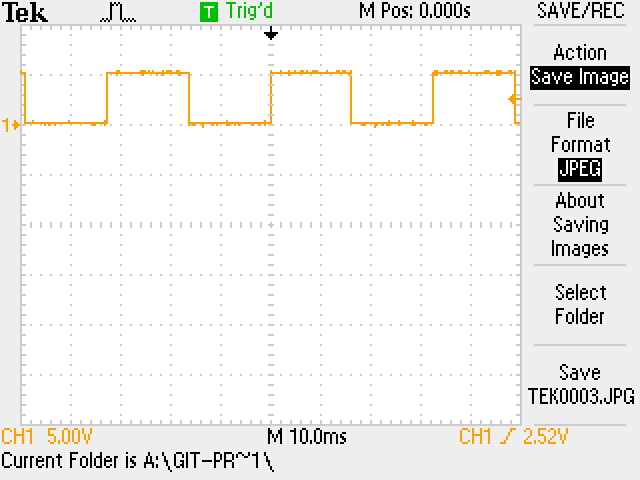
\includegraphics[width=0.75\textwidth]{p3} 
\caption{Größter Teilerfaktor(16384*2), kleinste Frequenz ($\approx 31 Hz$)}
\label{fq}
\end{center}
\end{figure}

\clearpage

\section{Anhang}
\subsection{Selbstständigkeitserklärung}
Hiermit versichern wir, dass wir das Protokoll selbstständig erarbeitet haben. Dabei haben wir keine anderen als die im Literaturverzeichnis angegebenen Quellen und Hilfsmittel benutzt, sowie Zitate kenntlich gemacht. 
\listoffigures
\nocite{*}
\bibliography{Literatur}
\bibliographystyle{plain}
\end{document}